\clearpage

\begin{wrapfigure}{r}{0.45\textwidth}
  \vspace{-6em}
  \centering
  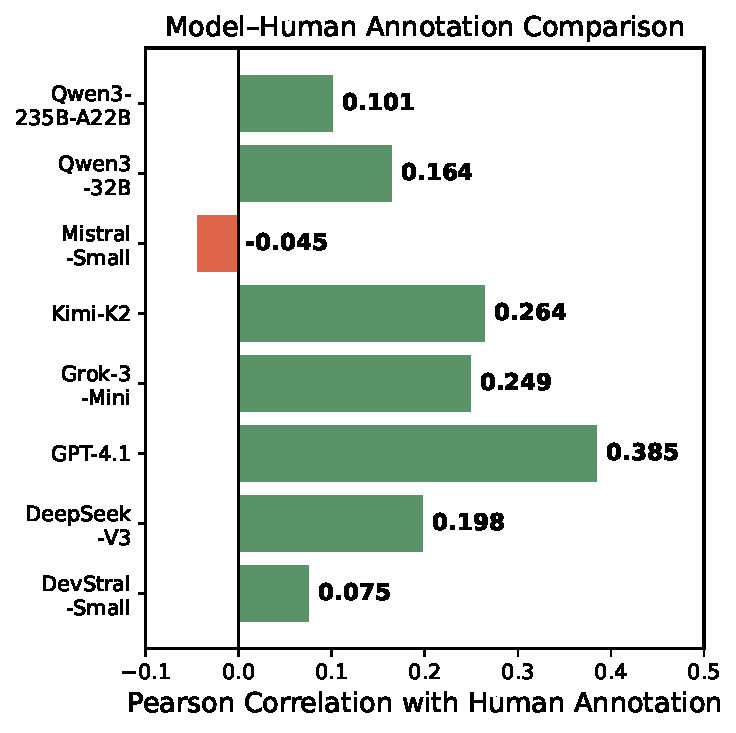
\includegraphics[width=0.44\textwidth]{images/annotation_correlation.pdf}
  \caption{Pearson correlation between human annotators and LLM-as-a-Judge evaluations across different models.}
  \label{fig:annotation-correlation}
  \vspace{-3em}
\end{wrapfigure}

\section{More on Experiments}

\subsection{LLM Annotation}
\label{app:llm-annotation}

Figure~\ref{fig:annotation-correlation} shows the Pearson correlation between human annotators and LLM-as-a-Judge evaluations across different models, based on 50 randomly sampled instances. The annotation prompt is available in Appendix \ref{app:task-annotation-prompt-for-single-server}. We observe that \texttt{GPT-4.1} and \texttt{Kimi-K2} achieve the highest overall correlation with human judgments. Considering cost efficiency, we deploy \texttt{Kimi-K2} locally for our annotation pipeline.

\subsection{Fine-Tuning Hyper-Parameters}\label{app:fine-tune-parameter}

We fine-tune models with \dataname using a super computing cluster, which is outfitted with NVIDIA H100 GPUs. The fine-tuning hyper-parameters can be found in Table \ref{tab:fine-tune hyperparameters}.

\begin{table}[htbp]
\small
\centering
% \vspace{-1em}
\caption{This table shows the hyper-parameters for supervised fine-tuning.}
% \vspace{1em}
\begin{tabular}{ll}
\toprule
\textbf{Hyper-parameter} & \textbf{Value} \\ \midrule
Tool-Call Template & Hermes \\
Learning Rate & $2 \times 10^{-5}$ \\
Number of Epochs & $2$ \\
Number of Devices & $8$ or $64$ \\
Per-device Batch Size & $1$ \\
Gradient Accumulation Steps & $8$ (8 GPUs) or $1$ (64 GPUs) \\
Effective Batch Size & $64$ \\
Optimizer & \texttt{Adamw} with $\beta s=(0.9,0.999)$ and $\epsilon=10^{-8}$\\
Deepspeed & zero3 \\
Max Sequence Length  & $32768$ \\ \bottomrule
\end{tabular}
% \vspace{-0.5em}
\label{tab:fine-tune hyperparameters}
\end{table}


\subsection{More on Ablation Studies}
\label{app:more-on-ablations}

Table~\ref{app:bfclv3-results-table-ablation} details the individual scores of the BFCL V3 benchmark for our ablation analysis. We observe that all extensions are meaningful in improving model performance.

\begin{table}[h!]
  \centering
  \caption{Ablation of \dataname Extensions on BFCL V3 Benchmark.}
  \label{app:bfclv3-results-table-ablation}
  \resizebox{\textwidth}{!}{%
  \begin{tabular}{@{}lllllll@{}}
\toprule
                                                     & \textbf{Overall} & \multicolumn{2}{c}{\textbf{Single Turn}} & \textbf{Multi Turn} & \multicolumn{2}{c}{\textbf{Hallucination}} \\
                                                     &                  & \textit{Non-live (AST)}        & \textit{Live (AST)}       &                     & \textit{Relevance}           & \textit{Irrelevance}          \\
                                                 \midrule
Qwen2.5-14B-Instruct                            & 57.69\%          & 83.38\%               & 73.70\%          & 19.75\%             & 83.33\%             & 68.46\%              \\
\quad+ Single Turn                                        & 60.16\%          & 87.50\%               & 66.86\%          & 34.38\%             & 72.22\%             & 46.88\%              \\
\quad\quad+ Irrelevance                          & 64.74\%          & 88.46\%               & 77.25\%          & 30.38\%             & 72.22\%             & 77.85\%              \\
\quad\quad\quad+ Diversify              & 64.56\%          & 86.06\%               & 76.90\%          & 32.50\%             & 72.22\%             & 75.45\%              \\
\quad\quad\quad\quad+ Multi-Turn & 65.09\%          & 85.42\%               & 76.01\%          & 35.25\%             & 72.22\%             & 75.96\%              \\ \bottomrule
\end{tabular}
  }
\end{table}
% \end{document}
